\documentclass{article}

% packages
\usepackage{amsmath, amsthm, thmtools, amsfonts, amssymb, luacode, catchfile, tikzducks, hyperref, ifthen}
\ifcsname c@kobocompile\endcsname
	\usepackage[a5paper, total={1072pt, 1448pt}, margin=10pt, includeheadfoot]{geometry} % set page margins
\else
	\usepackage[a4paper, margin=50pt, includeheadfoot]{geometry}
\fi
\usepackage[shortlabels]{enumitem}
\usepackage[skip=3pt, indent=0pt]{parskip}

% language
\usepackage[bidi=basic, layout=tabular, provide=*]{babel}
\ifcsname c@english\endcsname
	\babelprovide[main, import]{english}
\else
	\babelprovide[main, import]{hebrew}
	\babelprovide{rl}
\fi
%\babelfont{rm}{Libertinus Serif}
\babelfont{rm}[Renderer=Harfbuzz]{Libertinus Serif}
\babelfont{sf}{Libertinus Sans}
\babelfont{tt}{Libertinus Mono}

% style
\AddToHook{cmd/section/before}{\clearpage}	% Add line break before section
\linespread{1.3}
\setcounter{secnumdepth}{0}		% Remove default number tags from sections, this won't do well with theorems
\AtBeginDocument{\setlength{\belowdisplayskip}{3pt}}
\AtBeginDocument{\setlength{\abovedisplayskip}{3pt}}
\graphicspath{ {../images/} }

% operators
\DeclareMathOperator\cis{cis}
\DeclareMathOperator\Sp{Sp}
\DeclareMathOperator\tr{tr}
\DeclareMathOperator\im{Im}
\DeclareMathOperator\re{Re}
\DeclareMathOperator\diag{diag}
\DeclareMathOperator*\lowlim{\underline{lim}}
\DeclareMathOperator*\uplim{\overline{lim}}
\DeclareMathOperator\rng{rng}
\DeclareMathOperator\Sym{Sym}
\DeclareMathOperator\Arg{Arg}
\DeclareMathOperator\Log{Log}
\DeclareMathOperator\dom{dom}
\DeclareMathOperator\supp{Supp}
\DeclareMathOperator\var{Var}
\DeclareMathOperator\cov{Cov}

% commands
%\renewcommand\qedsymbol{\textbf{מש''ל}}
%\renewcommand\qedsymbol{\fbox{\emoji{lizard}}}
\newcommand{\Aa}[0]{\mathcal{A}}
\newcommand{\Bb}[0]{\mathcal{B}}
\newcommand{\CC}[0]{\mathbb{C}}
\newcommand{\Cc}[0]{\mathcal{C}}
\newcommand{\EE}[0]{\mathbb{E}}
\newcommand{\FF}[0]{\mathbb{F}}
\newcommand{\Ff}[0]{\mathcal{F}}
\newcommand{\Ii}[0]{\mathcal{I}}
\newcommand{\Gg}[0]{\mathcal{G}}
\newcommand{\Ll}[0]{\mathcal{L}}
\newcommand{\Mm}[0]{\mathcal{M}}
\newcommand{\NN}[0]{\mathbb{N}}
\newcommand{\Nn}[0]{\mathcal{N}}
\newcommand{\PP}[0]{\mathbb{P}}
\newcommand{\Pp}[0]{\mathcal{P}}
\newcommand{\QQ}[0]{\mathbb{Q}}
\newcommand{\RR}[0]{\mathbb{R}}
\newcommand{\Rr}[0]{\mathcal{R}}
\newcommand{\Ss}[0]{\mathcal{S}}
\newcommand{\TT}[0]{\mathbb{T}}
\newcommand{\Uu}[0]{\mathcal{U}}
\newcommand{\Vv}[0]{\mathcal{V}}
\newcommand{\Ww}[0]{\mathcal{W}}
\newcommand{\ZZ}[0]{\mathbb{Z}}
\newcommand{\acts}[0]{\circlearrowright}
\newcommand{\explain}[2] {
	\begin{flalign*}
		 && \text{#2} && \text{#1}
	\end{flalign*}
}
\newcommand{\maketitleprint}[0]{ \begin{center}
	%\begin{tikzpicture}[scale=3]
	%	\duck[graduate=gray!20!black, tassel=red!70!black]
	%\end{tikzpicture}	
	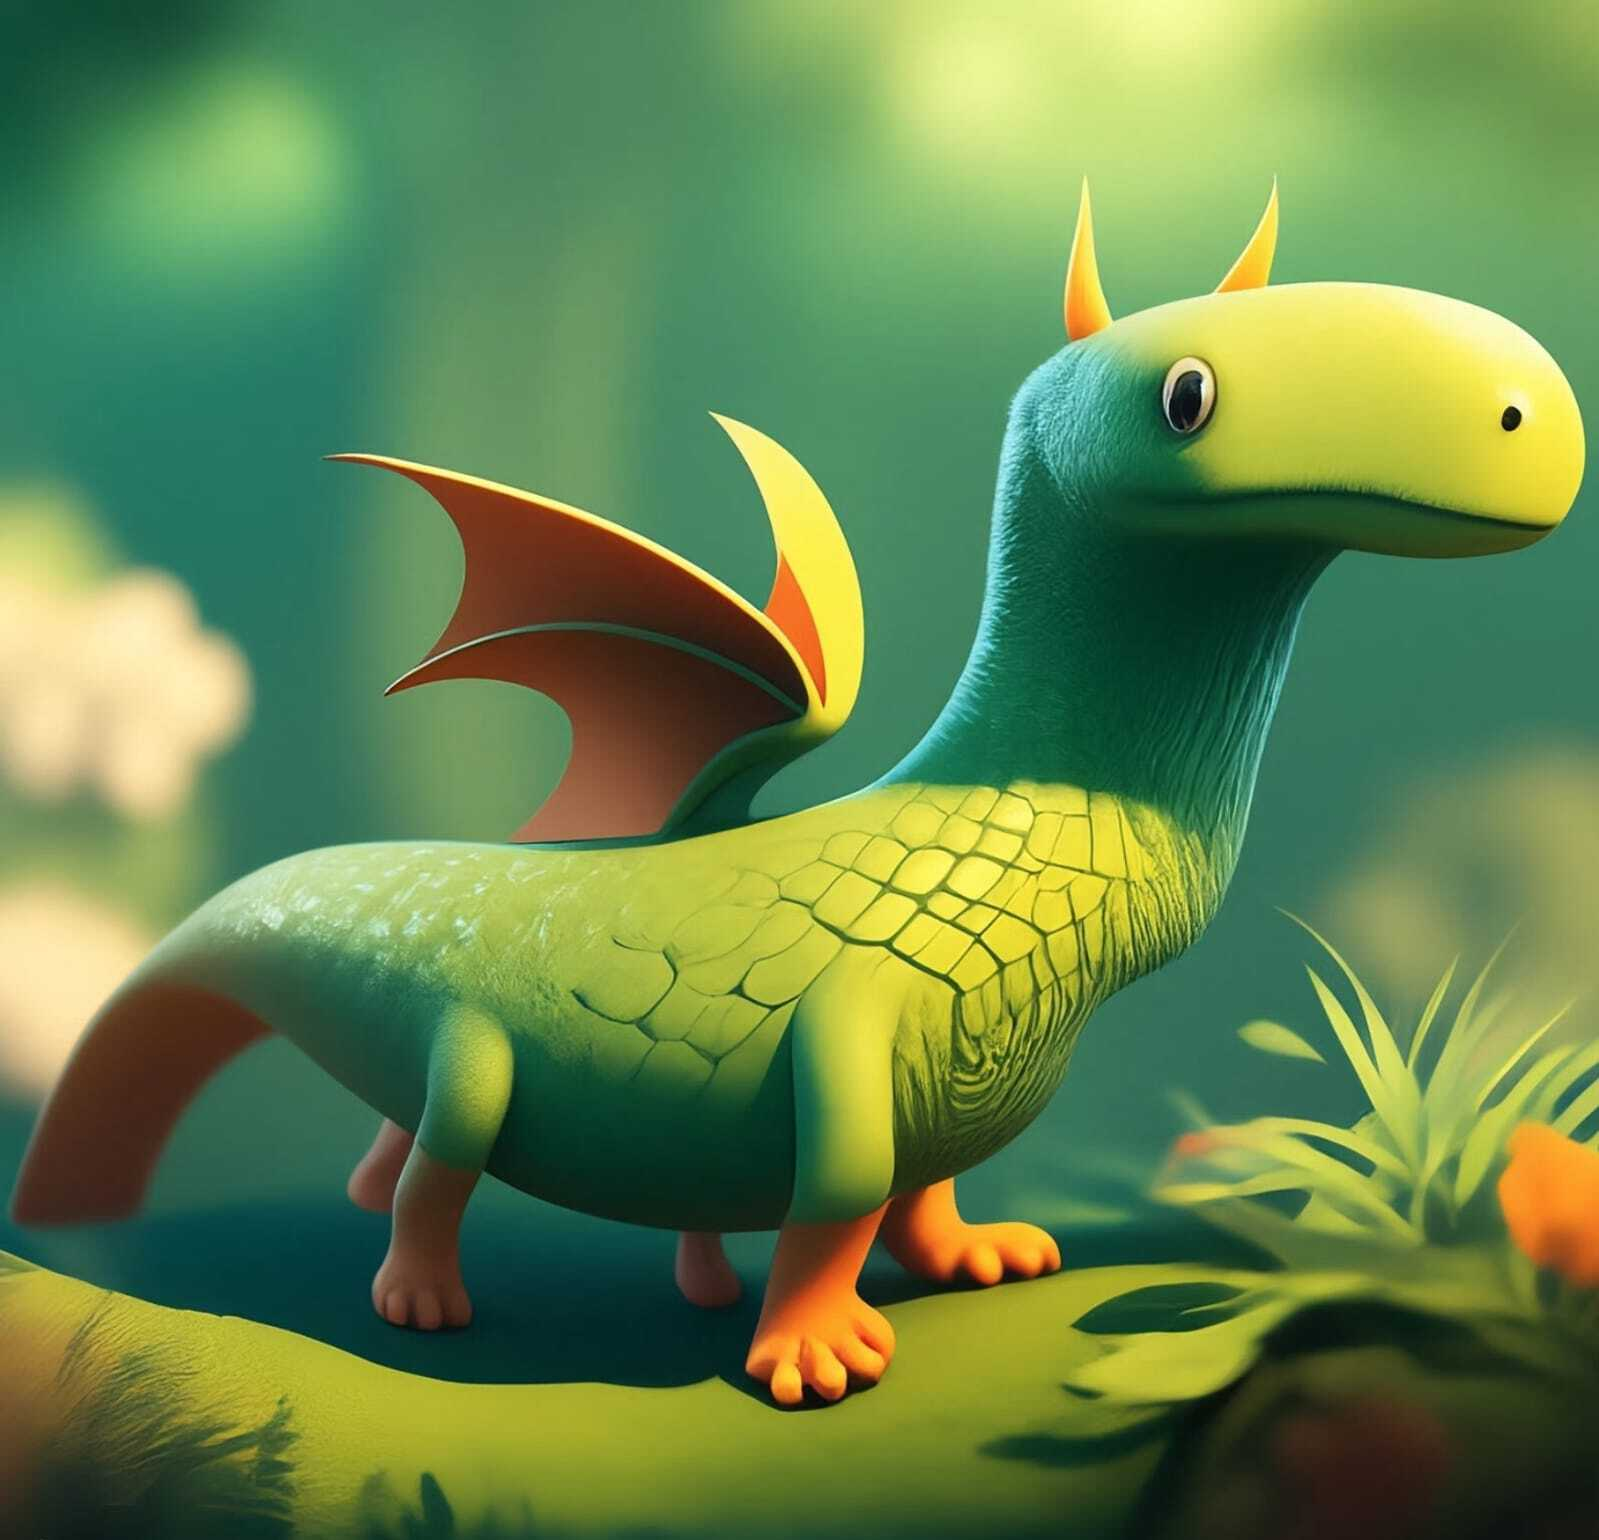
\includegraphics[width=6cm]{cover}
\end{center}
}

% theorem commands
\newtheoremstyle{c_remark}
	{}	% Space above
	{}	% Space below
	{}% Body font
	{}	% Indent amount
	{\bfseries}	% Theorem head font
	{}	% Punctuation after theorem head
	{.5em}	% Space after theorem head
	{\thmname{#1}\thmnumber{ #2}\thmnote{ \normalfont{\text{(#3)}}}}	% head content
\newtheoremstyle{c_definition}
	{3pt}	% Space above
	{3pt}	% Space below
	{}% Body font
	{}	% Indent amount
	{\bfseries}	% Theorem head font
	{}	% Punctuation after theorem head
	{.5em}	% Space after theorem head
	{\thmname{#1}\thmnumber{ #2}\thmnote{ \normalfont{\text{(#3)}}}}	% head content
\newtheoremstyle{c_plain}
	{3pt}	% Space above
	{3pt}	% Space below
	{\itshape}% Body font
	{}	% Indent amount
	{\bfseries}	% Theorem head font
	{}	% Punctuation after theorem head
	{.5em}	% Space after theorem head
	{\thmname{#1}\thmnumber{ #2}\thmnote{ \text{(#3)}}}	% head content

\ifcsname c@english\endcsname
	\theoremstyle{plain}
	\newtheorem{theorem}{Theorem}[section]
	\newtheorem{lemma}[theorem]{Lemma}
	\newtheorem{proposition}[theorem]{Proposition}
	\newtheorem*{proposition*}{Proposition}
	%\newtheorem{corollary}[theorem]{אין חלופה עברית}

	\theoremstyle{definition}
	\newtheorem{definition}[theorem]{Definition}
	\newtheorem*{definition*}{Definition}
	\newtheorem{example}{Example}[section]
	\newtheorem{exercise}{Exercise}[section]

	\theoremstyle{remark}
	\newtheorem*{remark}{Remark}
	\newtheorem*{solution}{Solution}
	\newtheorem{conclusion}[theorem]{Conclusion}
	\newtheorem{notation}[theorem]{Notation}
\else
	\theoremstyle{c_plain}
	\newtheorem{theorem}{משפט}[section]
	\newtheorem{lemma}[theorem]{למה}
	\newtheorem{proposition}[theorem]{טענה}
	\newtheorem*{proposition*}{טענה}
	%\newtheorem{corollary}[theorem]{אין חלופה עברית}

	\theoremstyle{c_definition}
	\newtheorem{definition}[theorem]{הגדרה}
	\newtheorem*{definition*}{הגדרה}
	\newtheorem{example}{דוגמה}[section]
	\newtheorem{exercise}{תרגיל}[section]

	\theoremstyle{c_remark}
	\newtheorem*{remark}{הערה}
	\newtheorem*{solution}{פתרון}
	\newtheorem{conclusion}[theorem]{מסקנה}
	\newtheorem{notation}[theorem]{סימון}
\fi

% Questions related commands
\newcounter{question}
\setcounter{question}{1}
\newcounter{sub_question}
\setcounter{sub_question}{1}

\ifcsname c@english\endcsname
	\newcommand{\question}[1][0]{
		\ifthenelse{#1 = 0}{}{\setcounter{question}{#1}}
		\section{Question \arabic{question}}
		\addtocounter{question}{1}
		\setcounter{sub_question}{1}
	}

	\newcommand{\subquestion}[1][0]{
		\ifthenelse{#1 = 0}{}{\setcounter{sub_question}{#1}}
		\subsection{Part \alph{sub_question}}
		\addtocounter{sub_question}{1}
	}
\else
	\newcommand{\question}[1][0]{
		\ifthenelse{#1 = 0}{}{\setcounter{question}{#1}}
		\section{שאלה \arabic{question}}
		\addtocounter{question}{1}
		\setcounter{sub_question}{1}
	}

	\newcommand{\subquestion}[1][0]{
		\ifthenelse{#1 = 0}{}{\setcounter{sub_question}{#1}}
		\subsection{סעיף \localecounter{letters.gershayim}{sub_question}}
		\addtocounter{sub_question}{1}
	}
\fi

% import lua and start of document
\directlua{common = require ('../common')}

\GetEnv{AUTHOR}

% headers
\author{\AUTHOR}
\date\today

\title{פתרון מטלה 06 --- תורת הקבוצות (80200)}

\begin{document}
\maketitle
\maketitleprint{}

\directlua{ Q_number = 2 }
\Question{}
\Subquestion{}
נוכיח כי הסדר $\langle \NN, \mid \rangle$ הוא סדר מבוסס היטב.
\begin{proof}
	תהי $\emptyset \ne B \subseteq \NN$ ויהי $\langle B, \mid \cap \mid \rangle$ הצמצום של הסדר. \\*
	$B$ היא תת־קבוצה של הטבעיים ולכן נוכל להסיק כי יש בה איבר מינימלי ביחס ל־$\le$. \\*
	נסמן איבר זה על־ידי $a$ ונראה כי הוא גם מינימלי על־פי $\mid$: \\*
	נבחין כי לכל איבר ב־$b \in B$ או ש־$a \mid b$, או ש־$b \mid a$, אבל במקרה זה ידוע גם כי $a \le b$ ולכן מתכונות המחלק נקבל כי $a = b$, או ששני הכיוונים לא מתקיימים, ונקבל כי $a$ מינימלי.
\end{proof}

\Subquestion{}
נמצא מינימום ומקסימום ב־$\langle \NN, \mid \rangle$.

עבור מינימום נבדוק ונראה כי $1$ מקיים את התנאים. \\*
ידוע כי $1 \mid a$ לכל $a \in \NN$ מתכונות הכפל.

נראה כי $0 \in \NN$ הוא מקסימום. \\*
על־פי הגדרת המחלק לכל $b \in \NN$ נקבל כי $0 = 0 \cdot b$ ולכן בהתאם $b \mid 0$, וכמובן ש־$0$ לא מחלק אף מספר על־פי הגדרה זו.
 
\Subquestion{}
נוכיח שב־$\langle \NN \setminus \{ 0 \}, \mid \rangle$ אין איברים מקסימליים.
\begin{proof}
	נניח בשלילה כי אכן יש איבר מקסימלי בקבוצה, ונסמנו על־ידי $t$, וידוע כי $1 \le t$, ולכן $t < 2t$. \\*
	נקבל כי $t \mid 2t$ אבל $2t \nmid t$ ובהתאם נובע כי $t$ לא מקסימלי, ובכלל אין מקסימום בסדר זה.
\end{proof}

\Subquestion{}
נוכיח כי ב־$\langle \NN \setminus \{ 1 \}, \mid \rangle$ אין מינימום.
\begin{proof}
	נניח בשלילה כי $t$ איבר מינימלי, וידוע כי $2 \le t$, ונבחן את $2t + 1$. \\*
	מהגדרת המחלק נקבל ישירות כי $t \nmid 2t + 1$ ובהתאם $t$ הוא לא מינימום, ובהתאם אין מינימום בקבוצה זו.
\end{proof}
נבדוק מיהם האיברים המינימליים בסדר. \\*
התשובה היא כלל הראשוניים, שכן כל מספר פריק ניתן לפרק לראשוניים, ומהסדר שהגדרנו נקבל כי הראשוניים מחלקים את הפריקים המורכבים מהם. \\*
לעומת זאת, אין מספר שמחלק את הראשוניים מלבד $1$, שאיננו בקבוצה, והמספרים עצמם, ולכן הם עומדים בהגדרת המינימלי.

\Question{}
תהי $A$ קבוצה. נוכיח כי הסדר החלקי $\langle \mathcal{P}(A), \subseteq \rangle$ מבוסס היטב אם ורק אם $A$ סופית.
\begin{proof}
	\textbf{כיוון ראשון:}
	נניח כי הסדר החלקי מבוסס היטב ונוכיח כי $A$ סופית. \\*
	נניח בשלילה כי $A$ לא סופית.
	יהי $a_0 \in A$ איבר כלשהו, $A$ אינסופית ולכן נוכל להסיק כי קיים כזה. נגדיר $A_1 = A \setminus \{ a_0 \}$. \\*
	ידוע כי $A_1$ אינסופית, ולכן נוכל להגדיר $a_1$ באופן דומה, וכך גם $A_2$ וכן הלאה. \\*
	אילו נקבל עבור $n \in \NN$ כלשהו כי $A_n$ לא קיים איבר $a_{n + 1} \in A$ נקבל סתירה לאינסופיות $A$ עצמה, ולכן נוכל להניח כי $\{ A_n \mid n \in \NN \}$ היא עצמה קבוצה אינסופית. \\*
	עוד נבחין כי $A_{n + 1} \subseteq A_n$ לכל $n \in \NN$. עתה נסיק מהעובדה שהסדר מבוסס היטב כדי לקבוע כי קיים איבר מינימלי לקבוצה זו, ולכן נקבל כי זהו גם מינימום. \\*
	קיבלנו אם כך שקיים $A_n$ כלשהו שהוא מינימלי, דהינו לא קיים $A_{n + 1} \subset A_n$ בסתירה לאינסופיות של $A$. \\*
	לכן נסיק כי $A$ היא סופית.

	\textbf{כיוון שני:}
	נניח כי $A$ סופית ונוכיח כי הסדר מבוסס היטב. \\*
	תהי $B \subseteq \mathcal{P}(A)$, אז קיים $C \in B$ לו יש מספר מינימלי של איברים, כלל הקבוצות הן סופיות ולכן מותר לנו להניח כן. \\*
	לכן מתכונות ההכלה לקבוצות סופיות נוכל להסיק כי לכל $D \in B$ או שאין יחס בין $C$ ו־$D$, או ש־$C \subseteq D$, ואילו $D \subseteq C$ אז גם $|D| \le |C|$ וידוע גם $|C| \le |D|$ ונקבל $C = D$,
	ומצאנו כי אכן $C$ מינימלית ובהתאם הסדר מבוסס היטב.
\end{proof}

\directlua{ Q_number = 7 }
\Question{}
נמצא סדרים חלקיים $\langle A, \le_A \rangle, \langle B, \le_B \rangle$ כך שקיימים שיכונים $f : \langle A, \le_A \rangle \to \langle B, \le_B \rangle$
וגם $g : \langle B, \le_B \rangle \to \langle A, \le_A \rangle$ אבל שגם $\langle A, \le_A \rangle \not\cong \langle B, \le_B \rangle$

נגדיר $A = \RR_{>0}$ ו־$B = \RR \cup \{ m\}$ ונגדיר $\le_A = \le_\RR, \le_B = \le_\RR \cup \{ \langle m, x \rangle \mid x \in \RR \}$. \\*
עוד נגדיר גם
\[
	f(x) = x,
	\qquad
	g(x) = \begin{cases}
		e^x + 1 & x \in \RR \\
		1 & x = m
	\end{cases}
\]
נשים לב כי $x \le_A y \iff x \le_B y$ ולכן $f$ היא שיכון. \\*
עבור $x, y \in B$ נקבל כי $x \le y \iff 1 \le e^x + 1 \lor e^x \le x^y$ ומצאנו כי זהו גם שיכון. \\*
למרות זאת בעוד ל־$B$ יש איבר מינימלי, ל־$A$ אין, ולכן נוכל להסיק כי הם לא איזומורפיים.

\Question{}
נגדיר
\begin{align*}
	& \langle \NN, \trianglelefteq \rangle,
	& \trianglelefteq = \{ \langle m, n \rangle \in \NN^2 \mid n = 0 \lor 0 < m \le n \} \\
	& \langle X, \preceq \rangle,
	& X = \{ p^n \mid n \in \NN_{>0}, p \text{ is prime}\}, \preceq = \{ \langle p^n, q^m \rangle \mid p < q \lor (p = q \land n \le m) \}
\end{align*}

\Subquestion{}
נוכיח כי אלו הם סדרים טובים ונבדוק אם הם איזומורפיים.
\begin{proof}
	נתחיל ב־$\langle \NN, \trianglelefteq \rangle$. \\*
	נבחין כי הסדר הוא רפלקסיבי, שכן עבור $0$ נקבל $n = 0$ ועבור $n > 0$ נקבל $0 < n \le n$. \\*
	נבחין כי הסדר גם אנטי־סימטרי, שכן יהיו שני מספרים $n \ne m$, אז אם $n = 0$ אז $m \trianglelefteq n$, אם $m = 0$ אז $n \trianglelefteq m$ ובכל מצב אחר $n < m$ או $m < n$ ובהתאם הסדר מתקיים לאחד הכיוונים תמיד. \\*
	מצאנו כי הסדר הוא סדר קווי, עתה נראה כי הוא גם מבוסס היטב.
	תהי $A \subseteq \NN$ ונבחן את $\langle A, \trianglelefteq \rangle$, זוהי תת־קבוצה של הטבעיים ולכן קיים איבר מינימלי $a$, ואם $a = 0$ אז ב־$A \setminus \{ a\}$ יש איבר מינימלי או שהקבוצה ריקה.
	אם הקבוצה ריקה אז מצאנו איבר מינימלי, ואם היא לא ריקה וגם $a = 0$ אז נגדיר את $a$ מחדש להיות המינימלי השני. \\*
	בכל מקרה נקבל כי $0 < a$ ולכן לכל מספר $b \in A$ נקבל כי אם $a \le b$ אז גם $a \trianglelefteq b$ ואם $b = 0$ אז מההגדרה גם $a \trianglelefteq b$, וקיבלנו כי $a$ אכן מינימלית. 
	בהתאם נובע כי $\langle \NN, \trianglelefteq \rangle$ היא סדר טוב.

	נעבור עתה להוכיח כי $\langle X, \preceq \rangle$ הוא סדר טוב אף הוא. \\*
	מההגדרה נובע ישירות כי הסדר הוא רפלקסיבי, נבדוק שלמות.
	יהיו $p^n, q^m$, ונניח כי $p^n \ne q^m$, אז או ש־$p \ne q$ ולכן הסדר מתקיים לאחד הכיוונים בהגדרה, או ש־$p = q$ ולכן נובע כי $m \ne n$ ושוב הוא מתקיים לאחד הכיוונים בהכרח.
	מצאנו כי זהו יחס קווי, עתה נוכיח סדר טוב.
	תהי $Y \subseteq X$ קבוצה לא ריקה, ונבחר קבוצה חדשה $Z = \{ p \mid p^n \in Y \}$, זוהי קבוצה של ראשוניים ובפרט של טבעיים, ולכן נוכל לבחור מינימום ביחס לסדר הטבעיים, נסמנו $p$. \\*
	נבחן את $Y^* = \{ p^n \mid n \in \NN_{>0}, p^n \in Y \}$, ובקבוצה זו קיים מינימלי כמובן ישירות מההגדרה, ולכן נקבע $p^n$ להיות מינימלי זה. \\*
	נחזור עתה לבחון את $Y$ עצמה, ונבחין כי לכל $q^m$ בקבוצה זו או $p \ne q$ ולכן גם $p < q$ ונקבל $p^n \preceq q^m$ או ש־$p = q$ ולכן $n \le m$ ועדיין נקבל כי $p^n \preceq q^m$ וקיבלנו כי יש איבר מינימלי ולכן הסדר הוא טוב.
\end{proof}
נבחין כי הסדרים לא איזומורפיים, שכן $2^n \preceq 3$ לכל $n$ טבעי ולכן ניאלץ לקבוע $f(3) = 0$ כדי שיתקבל $f(2^n) \le f(3)$, אבל גם $3^n \preceq 5$ לכל $n \in \NN$ ולא נוכל לייצג זאת על־ידי הסדר $\trianglelefteq$.

\Subquestion{}
נמצא את קבוצת המספרים שאינם עוקבים לאף מספר בכל קבוצה.

בסדר $\langle \NN, \trianglelefteq \rangle$
נראה כי לכל $n > 1$ נוכל לבחור $n - 1$ והוא יהווה עוקב עבורו, לכן רק $0, 1$ חשודים.
נבחין כי $1 \trianglelefteq 0$ ולכן $1$ לא עוקב לאף מספר.
ראינו כי לכל $n$ מתקיים $n \trianglelefteq 0$ ולכן $0$ הוא לא עוקב לאף איבר.

נבחן עתה את $\langle X, \preceq \rangle$, ונטען כי $\{ p^1 \mid p \text{ is prime}, p > 2 \}$ היא קבוצת האיברים שהם לא עוקבים לאף מספר. \\*
יהי $p$ כלשהו, ונבחר $q < p$ ראשוני קודם לו בקבוצת הראשוניים, אז נראה כי $q^n \preceq p$ לכל $n \in \NN$, ולכן נוכל להסיק כי $p^1$ לא עוקב לאף איבר.
בתהליך ההוכחה הראינו כי קבוצת איברים זו מכילה את כל האיברים שאינם עוקבים בלבד.

\Subquestion{}
נמצא $A, B \subseteq \RR$ כך שיתקיים
\[
	\langle A, \le_\RR \rangle \cong \langle \NN, \trianglelefteq \rangle,
	\qquad
	\langle B, \le_\RR \rangle \cong \langle X, \preceq \rangle,
\]

נגדיר $A = \{1\} \cup \{ 1 - \frac{1}{n} \mid n \in \NN \}, B = \{ n + \frac{1}{k} \mid n \text{ is prime}, k \in \NN_{>0} \}$ \\*
נגדיר $f : \NN \to A$ על־ידי
\[
	f(n) = \begin{cases}
		1 & n = 0 \\
		1 - \frac{1}{n} & n > 0
	\end{cases}
\]
לכן נקבל $n \trianglelefteq 0 \iff f(n) \le f(0) \iff 1 - \frac{1}{n} \le 1$, וגם $n \trianglelefteq m \iff 0 < n \le m \iff 0 < 1 - \frac{1}{n} \le 1 - \frac{1}{m} \iff f(n) \le f(m)$.
מצאנו כי זהו שיכון ונשאר להוכיח כי הוא על, אך למעשה הגדרנו את הקבוצה בהתאם לתמונת $f$ ולכן היא על, ונקבל כי מתקיימת איזומורפיה.

נעבור ל־$B$, ונגדיר $g : \langle X, \preceq \rangle \to \langle B, \le_\RR\rangle$ על־ידי
\[
	g(p^n) = p + 1 - \frac{1}{n + 1}
\]
אילו $p, q$ ראשוניים שונים אז $p^n \preceq q^m$ לכל $m, n$, וגם $p + 1 - \frac{1}{n + 1} \le p + 1 \le q \le q + 1 - \frac{1}{m + 1}$ ונקבל $g(p^n) \le g(q^m)$.
אילו $n \le m$ אז $p^n \preceq q^m$ ובהתאם $-\frac{1}{n + 1} \le -\frac{1}{m + 1}$ ונקבל כי $g(p^n) \le g(p^m)$, ומצאנו כי זהו אכן שיכון.
גם במקרה זה הקבוצה הוגדרה להיות תמונת השיכון ולכן היא על בהגדרתה ונקבל כי ישנה איזומורפיה.

\end{document}
